\documentclass[sigconf,nonacm]{acmart}
\usepackage{booktabs}
\usepackage{multirow}
\usepackage{graphicx}
\usepackage{xcolor}
\usepackage{tikz}
\usetikzlibrary{positioning,arrows.meta,shapes.geometric,fit,calc}

\setlength{\emergencystretch}{3em}
\hyphenpenalty=100

\newcommand{\sysname}{\textsf{GraphR}}

% Remove ACM-specific metadata for preprint
\settopmatter{printacmref=false}
\renewcommand\footnotetextcopyrightpermission[1]{}
\pagestyle{plain}
\begin{document}

\title{{\normalfont\sysname{}}: Structure-Aware Multi-Context Embeddings and Retrieval for Binary Function Name Recovery}

\author{Ananta Dian Pradipta}
\affiliation{%
  \institution{New Jersey Institute of Technology}
  \city{Newark}
  \state{NJ}
  \country{USA}
}
\email{adp232@njit.edu}

\author{Robert Blacha}
\affiliation{%
  \institution{New Jersey Institute of Technology}
  \city{Newark}
  \state{NJ}
  \country{USA}
}
\email{rb97@njit.edu}

\author{Zhihao Lin}
\affiliation{%
  \institution{New Jersey Institute of Technology}
  \city{Newark}
  \state{NJ}
  \country{USA}
}
\email{zl527@njit.edu}

\author{Haotian Zhang}
\affiliation{%
  \institution{New Jersey Institute of Technology}
  \city{Newark}
  \state{NJ}
  \country{USA}
}
\email{haotian.zhang@njit.edu}

\begin{abstract}
Recovering function names from stripped binaries is critical for reverse engineering, malware analysis, and vulnerability research. Recent systems for this task increasingly rely on billion-parameter LLM backbones. On our evaluation setup, we show a small, structure-aware encoder can match or outperform them. We present \sysname{}, a graph neural network-based system that learns function representations by fusing multiple context sources (external library calls, callee signatures, and caller signatures) through a cascaded gated fusion mechanism with conditional bypass. Our ablation study shows that external-call information alone improves in-distribution performance but reduces cross-project generalization by 4.3 points. Adding callee and caller context offsets this effect and improves disambiguation. We further show that self-supervised pre-training (MLM plus contrastive learning on O0/O2 pairs of the same function) paired with sufficient encoder capacity (we use 32M parameters; smaller variants benefit less from pre-training) delivers the largest single ablation gain: \textbf{+0.13 cross-project F1}. In our experiments, nearest-neighbor retrieval over encoder embeddings outperformed the autoregressive decoder on unseen packages, improving exact match by 4.7 points without additional training. This result suggests that, for our model and dataset, embedding quality was more important than the decoding strategy. Evaluated on 300{,}013 functions from 77 packages, \sysname{} achieves 0.770 F1 on a held-out test set (13{,}559 functions) and \textbf{0.718 F1} across 4 completely unseen packages (10{,}467 functions), outperforming the released SYMGEN checkpoint (0.45), an end-to-end SYMGEN+LoRA reproduction on the same 300K training set (0.66), BLens (0.46 reported), and a StarCoder-3B zero-shot baseline (0.65) while using only 25M parameters, over 1{,}000$\times$ smaller than SYMGEN's CodeLlama-34B.
\end{abstract}

\keywords{binary analysis, function name recovery, graph neural networks, gated fusion, retrieval-augmented inference}

\maketitle
\hypersetup{colorlinks=true,linkcolor=blue,citecolor=blue,urlcolor=blue}

% ============================================================================
\section{Introduction}
\label{sec:intro}

Software reverse engineering requires analysts to understand compiled binary programs without access to source code. Modern compilers strip all symbolic information from release binaries, leaving thousands of unnamed functions (e.g., \texttt{sub\_4a30}) that must be manually identified. Recovering meaningful function names dramatically accelerates program comprehension.

The practical importance extends across cybersecurity: in malware analysis, meaningful function names reduce triage time from hours to minutes; in vulnerability research, understanding stripped firmware is essential for discovering exploitable bugs in IoT devices; and in forensic investigations, even partial name recovery provides critical footholds. Commercial tools such as IDA Pro and Ghidra provide manual annotation workflows but cannot automatically recover names for arbitrary functions.

Prior work has explored statistical approaches~\cite{debin}, graph neural networks~\cite{nero}, language model pre-training~\cite{symlm}, and LLM fine-tuning~\cite{symgen}. However, two challenges remain underexplored: (1)~how to effectively combine multiple contextual sources without degrading generalization, and (2)~whether autoregressive generation is the right output paradigm, given that function names are drawn from a relatively small vocabulary of real names.

We address these with \sysname{}, a graph neural network system that lifts stripped binaries to BAP intermediate representation, encodes each function's control flow graph with a GAT-based encoder, and fuses multiple sources of inter-procedural context through a cascaded gated mechanism with conditional bypass. Self-supervised pretraining (masked language modeling and contrastive learning) with partial embedding transfer further strengthens the encoder representations. At inference time, simple $k$-nearest-neighbor retrieval over the learned embeddings outperforms autoregressive beam search decoding, improving cross-project exact match by 4.7 percentage points with zero retraining.

Evaluated on 300{,}013 functions from 77 packages, \sysname{} achieves 0.770 F1 on a held-out test set and \textbf{0.718 F1} across 4 unseen packages, leading the released SYMGEN~\cite{symgen} checkpoint (0.45), an end-to-end SYMGEN+LoRA reproduction (0.66), BLens~\cite{blens} (0.46 reported), and a StarCoder-3B zero-shot baseline (0.65). In summary, we make the following contributions:

\begin{itemize}
    \item We propose \sysname{}, a GNN-based system for binary function name recovery that uses staged gated fusion to combine multiple context sources. This 3-stage architecture sequentially fuses external library calls, callee signatures, and caller signatures with conditional bypass, where each stage is skipped when the corresponding context is absent. Our ablation study reveals the \emph{ext-call paradox}: external call information alone degrades cross-project generalization by 4.3 percentage points, while adding inter-procedural callee/caller context resolves this and improves cross-project EM by 12.8 percentage points.

    \item We present an empirical analysis showing that $k$-nearest-neighbor retrieval over encoder embeddings outperforms autoregressive decoding by +2.0pp test EM and +4.7pp cross-project EM with zero retraining. This finding, consistent with kNN-LM~\cite{knnlm}, demonstrates that for our encoder architecture, representation quality is the primary bottleneck rather than the decoding strategy.

    \item We demonstrate that a compact, structure-aware encoder can match or outperform billion-parameter LLM baselines: \sysname{}'s 32M parameters are over 1{,}000$\times$ fewer than SYMGEN's CodeLlama-34B backbone, and it serves predictions in single-digit milliseconds per function, an order of magnitude faster than autoregressive 34B-LLM decoding, making \sysname{} practical for interactive reverse-engineering.

    \item We show that self-supervised pre-training (MLM plus contrastive learning on O0/O2 pairs) paired with sufficient encoder capacity delivers our \textbf{largest single ablation gain: +0.13 cross-project F1}. Partial embedding transfer (84.4\% match) lets the pre-training generalize across dataset evolutions.

    \item We advance the state of the art in cross-project function name recovery, achieving 0.770 F1 on a held-out test set (13{,}559 functions) and \textbf{0.718 F1} across 4 completely unseen packages (10{,}467 functions), beating the released SYMGEN~\cite{symgen} checkpoint (0.45), an end-to-end SYMGEN+LoRA reproduction on the same 300K training data (0.66), BLens~\cite{blens} (0.46 reported), and a StarCoder-3B zero-shot baseline (0.65). On a matched 8{,}062-function subset we lead SYMGEN+LoRA by $+0.10$ F1 / $+26$pp EM. Self-supervised pretraining with partial embedding transfer contributes $+0.13$ cross-project F1. Our code and dataset are publicly available at \href{https://github.com/ananta-pradipta/stripped-binary-name-recovery}{\textcolor{blue}{https://github.com/\allowbreak{}ananta-pradipta/\allowbreak{}stripped-binary-name-recovery}}.
\end{itemize}

% ============================================================================
\section{Background and Motivation}
\label{sec:background}

\subsection{Problem Definition}
\label{sec:problem}

Given a stripped binary $B$ containing $n$ functions $\{f_1, \ldots, f_n\}$, where each $f_i$ is represented by its control flow graph $G_i = (V_i, E_i)$ with basic blocks as nodes, the goal is to predict a human-readable name $\hat{n}_i$ matching the developer-assigned name $n_i$. Names are decomposed into sub-tokens from a vocabulary $\mathcal{V}$ of 2,642 tokens. Each function may have external library calls $\mathcal{E}_i$, callee signatures $\mathcal{C}_i^{ee}$, and caller signatures $\mathcal{C}_i^{er}$; these are optional (approximately 70\% of functions have no external calls). We evaluate on x86-64 ELF binaries at O0 and O2 optimization levels.

\subsection{Challenges}
\label{sec:challenges}

Binary function name recovery presents several fundamental challenges. \textbf{Token collision}: after instruction-type tokenization, many structurally different functions share similar token distributions, motivating multi-context fusion. \textbf{Mode collapse}: naively incorporating context causes 47\% of predictions to collapse to a single name; our conditional bypass addresses this. \textbf{Cross-project gap}: BLens~\cite{blens} drops from 0.79 to 0.46 F1 on unseen packages; our ext-call paradox reveals that external calls alone \emph{hurt} generalization by 4.3pp. \textbf{O0/O2 gap}: O0 binaries produce many wrapper functions with 70\% token overlap, yielding 41.5\% vs.\ 69.8\% EM.

\subsection{External Calls}
\label{sec:external}
External calls exist in a program in order to allow for programs to use common library functions without needing to duplicate those functions across multiple binaries and to allow for updating libraries to be handled separately from updating individual programs. For the linker to be able to link a binaries external calls to the function in a loaded library (.dll in windows and .so in linux), it must retain the information of the function's name to link it to the appropriate function in a loaded library, even when that binary is stripped, optimized or even obfuscated. While other state of the art function name predictors handle all call instructions as the same token, GraphR is able to extract two vital pieces of information from separately collecting and analyzing the external calls within a function:

\begin{enumerate}
    \item The called external functions within an unnamed function, providing context on what the function is attempting to accomplish. % Robert: This is an example I am considering adding if the item is not clear: For example, a function that calls the external functions of socket(), listen(), or bind() is clearly related to networking, information that would otherwise be lost by handling external function calls as unnamed function calls
    \item The calling context of a function by reference to its callers and callees external function calls, allowing for functions without external function calls to gain the benefit from (1). 
    % Robert: This is an example I am considering adding if the item is not clear: This is best exemplified in a function that while lacking external function calls, is called by a function that calls open() and read(), and itself calls the functions write() and close(). In this example the information of the function working on a file is provided by considering the context of its callers and callees external function calls.
\end{enumerate}

\subsection{Related Work and Our Motivations}
\label{sec:related}

\textbf{Function Name Recovery.}
He et al.~\cite{debin} introduced DeBin, using probabilistic graphical models on BAP-IR to predict debug information. David et al.~\cite{nero} proposed NERO, using GNNs on call graphs (F1=0.455), but only for functions \emph{with} external calls, a limitation since 70\% of functions have none. Jin et al.~\cite{symlm} presented SymLM, pre-training on micro-execution traces and fusing caller/callee context (F1=0.585), but requiring dynamic analysis. Al-Kaswan et al.~\cite{blens} introduced BLens with ensemble embeddings (cross-project F1=0.46). Xu et al.~\cite{symgen} fine-tuned CodeLlama with LoRA (cross-project F1=0.38 after deduplication). Jiang et al.~\cite{beyondclass} and GenNm~\cite{gennm} applied domain-adapted LLMs. Unlike recent LLM-based approaches, we focus on a compact encoder and compare retrieval-based inference against autoregressive decoding.

\textbf{Binary Representation Learning.}
Xu et al.~\cite{gemini} pioneered GNN-based binary similarity with Gemini. Ding et al.~\cite{asm2vec} proposed Asm2Vec using random walks. Wang et al.~\cite{jtrans} introduced jTrans with jump-aware positional encoding. Pei et al.~\cite{trex} developed Trex for execution semantics. Zhu et al.~\cite{callee} showed +28\% F1 from pre-training in CALLEE, supporting our encoder pre-training approach. Zhu et al.~\cite{tygr} applied GNNs to type inference (TYGR), and He et al.~\cite{codenl} proposed semantics-oriented graph representations.

% ---- Figure 1: placed here so it renders at top of Overview page ----
\begin{figure*}[t!]
    \centering
    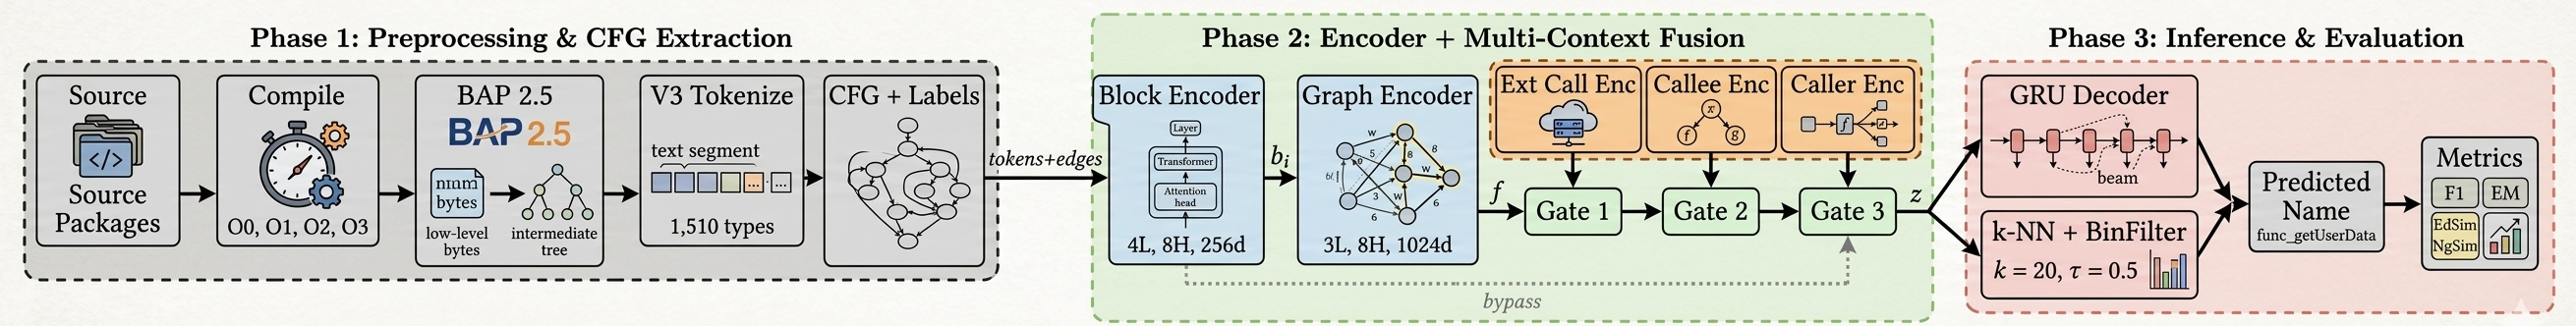
\includegraphics[width=\textwidth]{funcr_pipeline.png}
    \caption{End-to-end \sysname{} pipeline. Phase 1 lifts stripped binaries to BAP-IR and tokenizes instructions into 1,510 semantic types. Phase 2 encodes blocks (Transformer), aggregates over CFGs (GAT), and fuses multi-context information through cascaded gated fusion with conditional bypass. Phase 3 produces names via GRU beam search or $k$-NN retrieval.}
    \Description{End-to-end pipeline diagram showing three phases: preprocessing, encoder with multi-context fusion, and inference with evaluation.}
    \label{fig:pipeline}
\end{figure*}

\textbf{Retrieval-Augmented Methods.}
$k$NN-LM~\cite{knnlm} and $k$NN-MT~\cite{knnmt} showed that retrieval over hidden states can outperform neural models. Our setting differs: we retrieve \emph{complete} function names rather than interpolating token distributions, because function names are atomic labels, not compositional sequences.

% ============================================================================
\section{Overview}
\label{sec:overview}

\sysname{} follows a 3-stage encoder-decoder pipeline (Figure~\ref{fig:pipeline}): (1)~a block encoder tokenizes basic blocks into instruction-type tokens and produces per-block embeddings $\mathbf{b}_i \in \mathbb{R}^{512}$ via a Transformer~\cite{vaswani2017attention}; (2)~a GAT aggregates over the CFG to produce $\mathbf{f} \in \mathbb{R}^{1024}$, then cascaded gated fusion incorporates external calls, callee, and caller context with conditional bypass to produce $\mathbf{z} \in \mathbb{R}^{1024}$; (3)~either a GRU~\cite{gru} decoder or $k$-NN retrieval produces the function name. Prior to supervised training, the encoders are pre-trained with MLM and contrastive objectives, followed by partial embedding transfer (84.4\% matched by name).

% ============================================================================
\section{Detailed Design}
\label{sec:design}

\begin{figure*}[tb]
    \centering
    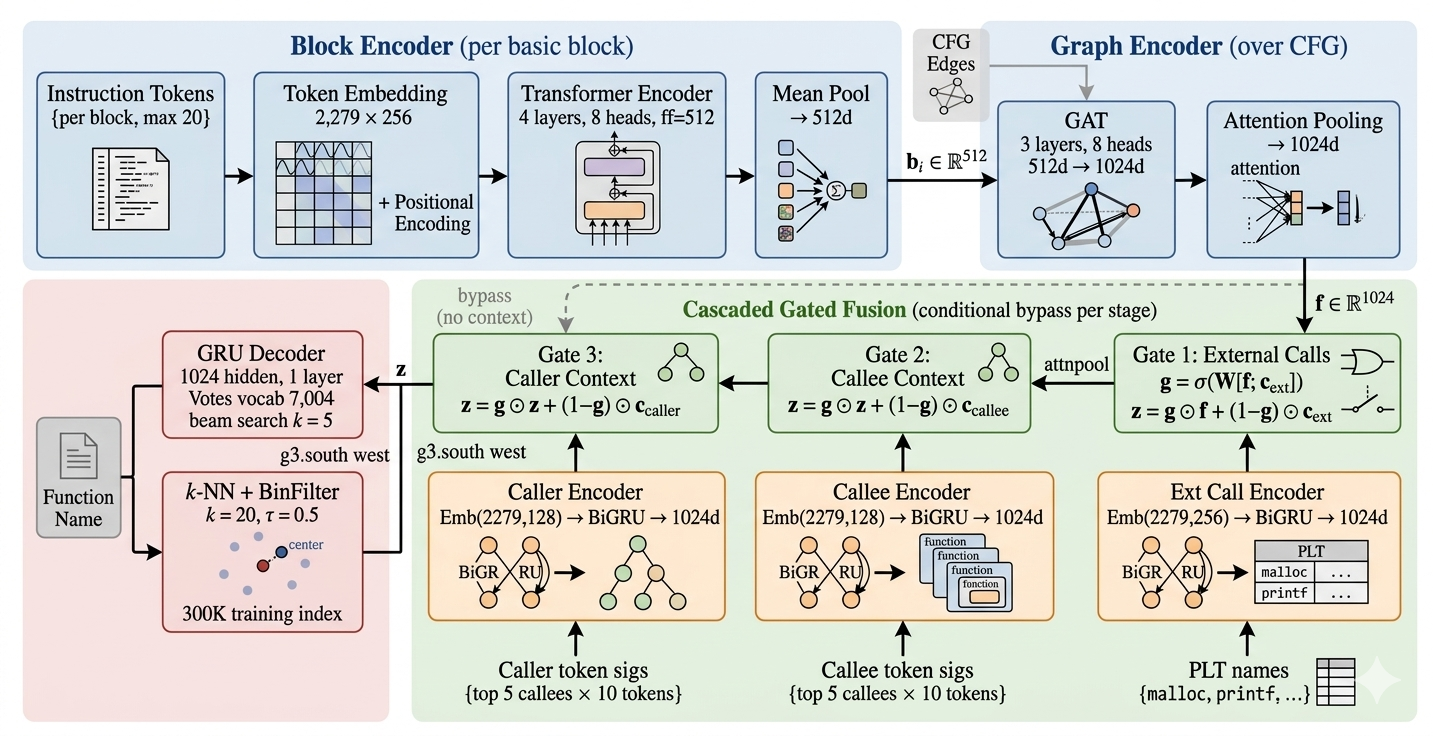
\includegraphics[width=0.95\textwidth]{funcr_architecture.png}
    \caption{Detailed model architecture. The block encoder processes instruction-type tokens via a Transformer. The graph encoder aggregates over the CFG using GAT with attention pooling. Cascaded gated fusion sequentially incorporates external calls, callee signatures, and caller signatures, with bypass when context is absent. The fused embedding feeds either a GRU decoder or $k$-NN retrieval.}
    \Description{Detailed model architecture diagram.}
    \label{fig:architecture}
\end{figure*}

\subsection{Preprocessing}

We compile 40 open-source packages at O0 and O2, lifting stripped binaries to BAP-IR~\cite{bap}. Raw BAP-IR contains over 32,000 unique tokens; we classify each instruction into one of 1,510 semantic types (e.g., \texttt{CALL\_malloc}, \texttt{MEM\_READ\_32}, \texttt{FLAG\_CF}, \texttt{ASSIGN\_ZERO}), reducing vocabulary by 95\% while preserving semantic distinctions. Ground-truth labels are extracted from debug binaries via \texttt{nm}. In O0 binaries, BAP lifts \texttt{endbr64; jmp target} sequences as separate functions; our preprocessing resolves these wrappers to the target function, raising O0 EM from 1.6\% to 41.5\%. Function names are tokenized into 2,642 sub-tokens using a 3-model voting tokenizer (Votes), reducing OOV by 95\% compared to BPE~\cite{bpe}.

\subsection{Block Encoder}

Each basic block contains up to 20 instruction-type tokens. We embed tokens via $\mathbf{E} \in \mathbb{R}^{2279 \times 256}$ with sinusoidal positional encodings, then apply a 4-layer Transformer (8 heads, $d_\text{ff}{=}512$). Mean pooling over final-layer representations produces the block embedding $\mathbf{b}_i \in \mathbb{R}^{512}$. We chose mean pooling over attention pooling after experimentation (0.58 vs.\ 0.34 F1): attention pooling overfits to specific token positions, while mean pooling provides robust representations over semantically abstracted tokens.

\subsection{Graph Encoder}

Given a function's CFG $G = (V, E)$ with block embeddings $\{\mathbf{b}_1, \ldots, \mathbf{b}_{|V|}\}$, we apply a 3-layer GAT~\cite{velivckovic2018graph} with 8 heads. Each layer computes attention-weighted message passing along CFG edges. An attention-based readout pools over blocks:
\begin{equation}
    \mathbf{f} = \sum_{i=1}^{|V|} \beta_i \cdot \mathbf{b}_i^{(L)}, \quad \beta_i = \frac{\exp(\mathbf{w}^\top \mathbf{b}_i^{(L)})}{\sum_{j} \exp(\mathbf{w}^\top \mathbf{b}_j^{(L)})}
\end{equation}
producing $\mathbf{f} \in \mathbb{R}^{1024}$.

\subsection{Cascaded Gated Fusion}
\label{sec:fusion}

The core architectural contribution is a 3-stage cascaded fusion:

\textbf{Stage 1: External Calls.} A BiGRU encodes library function names (e.g., \texttt{malloc}, \texttt{fprintf}) to produce $\mathbf{c}_\text{ext} \in \mathbb{R}^{1024}$. A sigmoid gate determines the balance:
\begin{equation}
    \mathbf{g} = \sigma(\mathbf{W}_g [\mathbf{f}; \mathbf{c}_\text{ext}] + \mathbf{b}_g)
\end{equation}
\begin{equation}
    \mathbf{z} = \begin{cases}
        \mathbf{g} \odot \mathbf{f} + (1 - \mathbf{g}) \odot \mathbf{c}_\text{ext} & \text{if has ext calls} \\
        \mathbf{f} & \text{otherwise (bypass)}
    \end{cases}
\end{equation}

\textbf{Stage 2: Callee Context.} For up to 5 internal callees, we extract 10-token signatures and encode via a separate BiGRU. Gated fusion with bypass updates $\mathbf{z}$.

\textbf{Stage 3: Caller Context.} Symmetrically encodes up to 5 caller signatures.

\textbf{Conditional bypass is critical.} Approximately 70\% of functions have no external calls. Without bypass, the gate learns a default output, causing 47\% of predictions to collapse to a single name.

\subsection{Self-Supervised Pre-training}

We pre-train the block encoder and graph encoder jointly with two objectives (Figure~\ref{fig:pretraining}):

\begin{enumerate}
    \item \textbf{Masked Language Model (MLM):} 15\% of instruction tokens are randomly masked. The MLM head predicts the original tokens from the block encoder's per-token embeddings (before pooling). This trains the block encoder to produce meaningful token-level representations.
    \item \textbf{Contrastive Learning:} The same function compiled at O0 and O2 should produce similar graph-level embeddings; different functions should produce dissimilar embeddings. We use contrastive loss on the graph encoder output. This trains both the block encoder and graph encoder to be invariant to optimization-level differences.
\end{enumerate}

After 10 epochs of pre-training on an A100 GPU (${\sim}$45 minutes), we perform partial embedding transfer: 84.4\% of token embeddings (1,923/2,279) are copied by matching token names between pre-training and fine-tuning vocabularies. The remaining 356 tokens are randomly initialized.

% ---- Figure 3: Self-supervised pretraining ----
\begin{figure}[t]
    \centering
    \resizebox{\columnwidth}{!}{%
    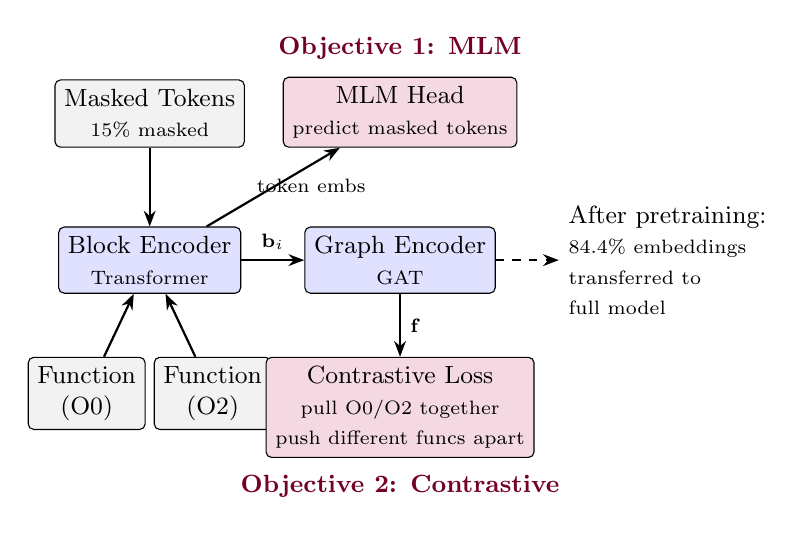
\begin{tikzpicture}[
        node distance=0.4cm and 0.5cm,
        box/.style={rectangle, draw, rounded corners=2pt, minimum height=0.55cm, align=center, font=\small},
        enc/.style={box, fill=blue!12, minimum width=1.6cm},
        loss/.style={box, fill=purple!15, minimum width=1.6cm},
        data/.style={box, fill=gray!10, minimum width=1.4cm},
        arr/.style={-{Stealth[length=2mm]}, thick},
        lbl/.style={font=\scriptsize},
    ]
    \node[enc] (be) {Block Encoder\\{\scriptsize Transformer}};
    \node[enc, right=0.8cm of be] (ge) {Graph Encoder\\{\scriptsize GAT}};
    \draw[arr] (be) -- node[above, lbl] {$\mathbf{b}_i$} (ge);
    \node[data, above=1.0cm of be] (masked) {Masked Tokens\\{\scriptsize 15\% masked}};
    \node[loss, above=1.0cm of ge] (mlm) {MLM Head\\{\scriptsize predict masked tokens}};
    \draw[arr] (masked) -- (be);
    \draw[arr] (be) -- node[above right, lbl, pos=0.3] {\scriptsize token embs} (mlm);
    \node[above=0.1cm of mlm, font=\small\bfseries, text=purple!60!black] {Objective 1: MLM};
    \node[data, below=0.8cm of be, xshift=-0.8cm] (o0) {Function\\(O0)};
    \node[data, below=0.8cm of be, xshift=0.8cm] (o2) {Function\\(O2)};
    \node[loss, below=0.8cm of ge] (ntxent) {Contrastive Loss\\{\scriptsize pull O0/O2 together}\\{\scriptsize push different funcs apart}};
    \draw[arr] (o0) -- (be);
    \draw[arr] (o2) -- (be);
    \draw[arr] (ge) -- node[right, lbl] {$\mathbf{f}$} (ntxent);
    \node[below=0.1cm of ntxent, font=\small\bfseries, text=purple!60!black] {Objective 2: Contrastive};
    \node[right=0.8cm of ge, font=\small, align=left] (transfer) {After pretraining:\\{\scriptsize 84.4\% embeddings}\\{\scriptsize transferred to}\\{\scriptsize full model}};
    \draw[arr, dashed] (ge.east) -- (transfer.west);
    \end{tikzpicture}%
    }
    \caption{Self-supervised pretraining. MLM trains the block encoder via masked token prediction. Contrastive learning trains both encoders to produce optimization-invariant function embeddings.}
    \Description{Pretraining diagram showing MLM and contrastive objectives.}
    \label{fig:pretraining}
\end{figure}

\subsection{Decoder and $k$-NN Inference}

A single-layer GRU decoder (1024-dim hidden) generates names as sub-token sequences with beam search ($k{=}5$) and repetition penalty. Training uses scheduled sampling~\cite{bengio2015scheduled} (teacher forcing 1.0$\to$0.3) and label smoothing~\cite{labelsmooth} (0.1).

For $k$-NN retrieval, at inference we encode the query function, retrieve the top-20 nearest training embeddings (datastore of 300{,}013 training functions) by cosine similarity, apply a \textbf{BinFilter} (cosine similarity $\geq 0.5$ in binary-level embedding space) to keep only retrievals from binaries similar to the query, and return the majority-voted name. If fewer than $k$ candidates survive, we fall back to the unfiltered top-$k$ retrieval. This $k$-NN + BinFilter ($\tau{=}0.5$) inference reaches F1 0.718 on the 4-package cross-project set and 0.770 on the held-out test set, without any retraining beyond the standard encoder checkpoint.

% ============================================================================
\section{Evaluation}
\label{sec:eval}

\subsection{Experimental Setup}

\begin{table}[t]
    \centering
    \caption{Dataset statistics.}
    \label{tab:dataset}
    \footnotesize
    \begin{tabular}{lr}
        \toprule
        \textbf{Metric} & \textbf{Value} \\
        \midrule
        Total packages / binaries & 77 / 851 \\
        Optimization levels & O0, O1, O2, O3 \\
        Training functions & 300{,}013 \\
        Validation / Test functions & 7{,}823 / 13{,}559 \\
        Cross-project functions (\textbf{4 unseen pkgs}) & 10{,}467 \\
        Instruction / Name / Ext-call vocab & 2,279 / 7{,}004 / 2{,}237 \\
        \bottomrule
    \end{tabular}
\end{table}

Table~\ref{tab:dataset} summarizes the dataset. We compile \textbf{77 packages} at O0, O1, O2, and O3. Data is split by binary (not function) to prevent leakage; 4 packages are held out entirely for cross-project evaluation.

We evaluate with \textbf{sub-token F1} (precision/recall over sub-tokens), \textbf{exact match (EM)}, \textbf{edit similarity} ($1 - \text{Lev}/\max$), and \textbf{n-gram similarity} (character 3-gram overlap).

\subsection{Ablation Study}

\begin{table}[t]
    \centering
    \caption{Ablation study. All models trained on the same 87K dataset for the ablation study.}
    \label{tab:ablation}
    \footnotesize
    \setlength{\tabcolsep}{4pt}
    \begin{tabular}{clccccc}
        \toprule
        \textbf{\#} & \textbf{Model} & \textbf{Params} & \textbf{Test F1} & \textbf{Test EM} & \textbf{XProj F1} & \textbf{XProj EM} \\
        \midrule
        2 & GAT + Decoder & 4.4M & 0.606 & 51.3\% & 0.364 & 24.1\% \\
        3 & + Ext Calls & 6.1M & 0.683 & 60.1\% & 0.320 & 19.8\% \\
        4 & + Callee/Caller & 8.0M & 0.781 & 72.3\% & 0.460 & 32.6\% \\
        5 & + Pretrain+Scale & 25M & 0.795 & 74.3\% & 0.593 & 48.5\% \\
        \bottomrule
    \end{tabular}
\end{table}

Table~\ref{tab:ablation} shows incremental contributions. \textbf{Model 2} (baseline) uses only the block encoder, graph encoder, and GRU decoder. \textbf{Model 3} adds external calls: test F1 improves +0.077 but cross-project EM \emph{drops} 4.3pp, revealing the ext-call paradox. \textbf{Model 4} adds callee/caller context, resolving the paradox: cross-project EM jumps +12.8pp. \textbf{Model 5} scales to 25M parameters with pre-training: cross-project F1 jumps +0.13, as the larger model eliminates cross-package contamination.

\textbf{The Ext-Call Paradox.} The Model 2$\to$3 transition reveals that external calls \emph{degrade} cross-project EM despite improving test F1. Many unrelated functions share similar library call patterns (e.g., \texttt{hash\_insert} and \texttt{tree\_add} both call \texttt{malloc} + \texttt{memcpy}). Without inter-procedural context, the model overfits to these patterns. Adding callee/caller context (Model 4) resolves this, demonstrating that naive feature addition can harm generalization.

\subsection{Main Results}

\begin{table}[t]
    \centering
    \caption{Main results: decoder vs.\ $k$-NN inference.}
    \label{tab:main}
    \footnotesize
    \begin{tabular}{lcccc}
        \toprule
        \textbf{Method} & \textbf{Test EM} & \textbf{Test F1} & \textbf{XProj EM} & \textbf{XProj F1} \\
        \midrule
        Decoder only (beam) & 70.6\% & 0.770 & 54.6\% & 0.673 \\
        $k$-NN unfiltered & 70.8\% & 0.770 & 56.1\% & 0.698 \\
        $k$-NN + BinFilter ($\tau{=}0.5$) & \textbf{70.8\%} & \textbf{0.770} & \textbf{57.0\%} & \textbf{0.718} \\
        \bottomrule
    \end{tabular}
\end{table}

Table~\ref{tab:main} shows $k$-NN with a binary-fingerprint filter outperforms the decoder on cross-project (+2.4pp EM, +0.045 F1) with zero retraining. The filter keeps retrieval candidates whose parent binary has at least Jaccard $\tau{=}0.5$ overlap in external-call vocabulary with the query binary, which reduces cross-package contamination.

We identify three decoder failure modes that $k$-NN eliminates: (1)~\textbf{hallucinated predictions} (43.8\% of decoder outputs are names absent from training); (2)~\textbf{error cascade} (one wrong sub-token corrupts all subsequent tokens); (3)~\textbf{unconstrained search space} ($2{,}642^{20}$ possible sequences vs.\ ${\sim}3{,}000$ real names).

\subsection{Cross-Project Analysis}

\begin{table}[t]
    \centering
    \caption{Per-package cross-project results. All 4 packages are completely excluded from training.}
    \label{tab:perpackage}
    \footnotesize
    \begin{tabular}{lrccc}
        \toprule
        \textbf{Package} & \textbf{Funcs} & \textbf{Dec.\ F1} & \textbf{$k$-NN F1} & \textbf{$k$-NN EM} \\
        \midrule
        nginx118 & 3{,}470 & 0.787 & \textbf{0.883} & 72.9\% \\
        angie    & 3{,}893 & 0.699 & \textbf{0.814} & 63.2\% \\
        tengine  &   554   & 0.685 & 0.738 & 66.8\% \\
        recutils & 2{,}550 & 0.296 & 0.343 & 24.0\% \\
        \midrule
        \textbf{Overall} & \textbf{10{,}467} & \textbf{0.673} & \textbf{0.718} & \textbf{57.0\%} \\
        \bottomrule
    \end{tabular}
\end{table}

Table~\ref{tab:perpackage} shows $k$-NN + binfilter improves all four packages. Nginx-family packages reach 0.74--0.88 F1 because they share substantial vocabulary with nginx training binaries; recutils stays at 0.343 F1 because its \texttt{rec\_*} / \texttt{recutl\_*} names share no sub-tokens with any training package.

\subsection{Comparison with Published Systems}

\begin{table}[t]
    \centering
    \caption{Comparison with published systems (cross-project F1).}
    \label{tab:comparison}
    \footnotesize
    \begin{tabular}{llcc}
        \toprule
        \textbf{System} & \textbf{Venue} & \textbf{Params} & \textbf{XProj F1} \\
        \midrule
        SYMGEN released~\cite{symgen} & NDSS 2025 & 34B & 0.450 \\
        SYMGEN + LoRA (our 300K) & NDSS 2025 & 34B & 0.663 \\
        BLens reported~\cite{blens} & USENIX Sec 2025 & ${\sim}200$M & 0.46 \\
        SymLM (BLens repro)~\cite{symlm,blens} & CCS 2022 & N/A & 0.277$^\ddagger$ \\
        LLM Zero-Shot (StarCoder-3B) & N/A & 3B & 0.654 \\
        \sysname{} (ours) & N/A & \textbf{32M} & \textbf{0.718} \\
        \bottomrule
    \end{tabular}
    \\[0.3em]
    \footnotesize$^\ddagger$Reported on Punstrip cross-project (different test set), reproduced by Benoit et al.~\cite{blens}.
\end{table}

\sysname{} leads all four baselines on the same 4-package cross-project set while being over 1{,}000$\times$ smaller than SYMGEN's CodeLlama-34B backbone. Doubling the LoRA fine-tuning data from 50\%-stratified (0.699) to full 300K (0.663) made SYMGEN worse, consistent with LoRA overfitting; we report the full-data number for fairness. On a matched 8{,}062-function subset with same \texttt{(package, name)} keys, \sysname{} leads SYMGEN+LoRA by $+0.10$ F1 / $+26$pp EM. SYMGEN wins only on recutils, whose source was plausibly in CodeLlama's pretraining corpus.

\textbf{Fairness disclaimer.} CodeLlama-34B and StarCoder-3B were pretrained on undisclosed but broad open-source corpora that almost certainly include the upstream repositories of every cross-project package we evaluate against. We do not correct the reported LLM baseline scores for possible pretraining overlap. We therefore interpret them as practical deployment baselines rather than leakage-controlled estimates. \sysname{}'s encoder is trained from scratch on BAP-IR with no exposure to source code or pretrained text embeddings, so its cross-project numbers genuinely measure generalization. The same caveat applies to BLens and SymLM literature numbers, which use Punstrip Debian binaries similarly well-represented in any large code corpus.

\begin{table}[t]
    \centering
    \caption{Computation cost comparison. \sysname{} trains in 2h 12m on a single A100 and serves predictions in $\sim$5\,ms per function.}
    \label{tab:cost-comparison}
    \footnotesize
    \begin{tabular}{lrr}
        \toprule
        \textbf{System} & \textbf{Params} & \textbf{Infer/fn} \\
        \midrule
        \textbf{\sysname{} (ours)} & \textbf{32M} & \textbf{\textasciitilde{}5 ms} \\
        SYMGEN + LoRA (full)       & 34B          & \textasciitilde{}200 ms \\
        SYMGEN (zero-shot)         & 34B          & \textasciitilde{}200 ms \\
        StarCoder-3B (zero-shot)   & 3B           & \textasciitilde{}80 ms \\
        \bottomrule
    \end{tabular}
\end{table}

\subsection{Significance and Error Analysis}

\begin{table}[t]
    \centering
    \caption{Error categorization on the test set (13{,}559 functions).}
    \label{tab:errors}
    \footnotesize
    \begin{tabular}{lrrrr}
        \toprule
        \textbf{Category} & \textbf{Dec.} & \textbf{Dec.\%} & \textbf{$k$-NN} & \textbf{$k$-NN\%} \\
        \midrule
        Correct & 6,671 & 74.3 & 6,850 & 76.3 \\
        Close (EdSim${>}$0.7) & 307 & 3.4 & 238 & 2.7 \\
        Hallucinated & 356 & 4.0 & 177 & 2.0 \\
        Wrong (seen name) & 654 & 7.3 & 758 & 8.4 \\
        Unseen target & 985 & 11.0 & 950 & 10.6 \\
        \bottomrule
    \end{tabular}
\end{table}

Table~\ref{tab:errors} categorizes test predictions. $k$-NN halves hallucinated predictions (4.0\%$\to$2.0\%) but trades them for wrong-seen errors (7.3\%$\to$8.4\%). The 11.0\% unseen-target functions are unsolvable by any recognizer, establishing a theoretical EM ceiling of ${\sim}$89\%. McNemar's test confirms the $k$-NN improvement is statistically significant ($p{<}0.001$) on both test and cross-project sets.

% ============================================================================
\section{Case Study}
\label{sec:casestudy}

\begin{table}[t]
    \centering
    \caption{Representative prediction examples. Correct predictions in \textbf{bold}; incorrect in \textit{italics}.}
    \label{tab:pred_examples}
    \footnotesize
    \resizebox{\columnwidth}{!}{%
    \begin{tabular}{llll}
        \toprule
        \textbf{Ground Truth} & \textbf{Decoder} & \textbf{$k$-NN} & \textbf{Category} \\
        \midrule
        \multicolumn{4}{l}{\textit{Both correct (shared gnulib functions):}} \\
        \texttt{xmalloc} & \textbf{\texttt{xmalloc}} & \textbf{\texttt{xmalloc}} & Both correct \\
        \texttt{set\_program\_name} & \textbf{\texttt{set\_program\_name}} & \textbf{\texttt{set\_program\_name}} & Both correct \\
        \texttt{xstrdup} & \textbf{\texttt{xstrdup}} & \textbf{\texttt{xstrdup}} & Both correct \\
        \texttt{version\_etc} & \textbf{\texttt{version\_etc}} & \textbf{\texttt{version\_etc}} & Both correct \\
        \texttt{usage} & \textbf{\texttt{usage}} & \textbf{\texttt{usage}} & Both correct \\
        \midrule
        \multicolumn{4}{l}{\textit{$k$-NN correct, decoder wrong:}} \\
        \texttt{hash\_pjw} & \textit{\texttt{hash\_insert}} & \textbf{\texttt{hash\_pjw}} & Decoder confused \\
        \texttt{quotearg\_buffer} & \textit{\texttt{quotearg\_n\_options}} & \textbf{\texttt{quotearg\_buffer}} & Decoder suffix error \\
        \texttt{close\_stdout} & \textit{\texttt{close\_stdout\_set}} & \textbf{\texttt{close\_stdout}} & Hallucinated suffix \\
        \texttt{trim2} & \textit{\texttt{trim\_trailing}} & \textbf{\texttt{trim2}} & Decoder composes \\
        \texttt{hard\_locale} & \textit{\texttt{locale\_charset}} & \textbf{\texttt{hard\_locale}} & Decoder wrong match \\
        \midrule
        \multicolumn{4}{l}{\textit{Decoder correct, $k$-NN wrong:}} \\
        \texttt{set\_program\_name} & \textbf{\texttt{set\_program\_name}} & \textit{\texttt{set\_prog\_name}} & $k$-NN truncated \\
        \texttt{c\_isspace} & \textbf{\texttt{c\_isspace}} & \textit{\texttt{c\_isdigit}} & $k$-NN neighbor \\
        \midrule
        \multicolumn{4}{l}{\textit{Both close (partially correct):}} \\
        \texttt{bfd\_pei\_swap\_aux\_in} & \textit{\texttt{bfd\_pex64i\_swap\_aux}} & \textit{\texttt{bfd\_coff\_swap\_aux}} & EdSim 0.86 \\
        \texttt{elf\_link\_hash\_traverse} & \textit{\texttt{elf\_link\_hash\_lookup}} & \textit{\texttt{elf\_link\_hash\_table}} & EdSim 0.82 \\
        \texttt{print\_str.part.0} & \textit{\texttt{print\_strs.part.0}} & \textit{\texttt{print\_str.isra.0}} & Off by one token \\
        \midrule
        \multicolumn{4}{l}{\textit{Both wrong (unseen target names; examples drawn from the broader test corpus):}} \\
        \texttt{diffutils\_cleanup} & \textit{\texttt{hash\_free}} & \textit{\texttt{xmalloc}} & Unseen name \\
        \texttt{datamash\_median} & \textit{\texttt{xmalloc}} & \textit{\texttt{set\_program\_name}} & Domain-specific \\
        \texttt{process\_cppi\_file} & \textit{\texttt{quotearg\_buffer}} & \textit{\texttt{xstrdup}} & Package-specific \\
        \texttt{csplit\_main\_loop} & \textit{\texttt{hash\_lookup}} & \textit{\texttt{close\_stdout}} & Package-specific \\
        \texttt{compute\_variance} & \textit{\texttt{xmalloc}} & \textit{\texttt{xrealloc}} & Stats function \\
        \bottomrule
    \end{tabular}%
    }
\end{table}

Table~\ref{tab:pred_examples} shows representative predictions across five categories. The first group illustrates shared gnulib functions both methods recover. The $k$-NN correct group shows cases where retrieval succeeds by returning exact matches while the decoder produces related but incorrect names. The decoder correct group shows rare cases where autoregressive generation outperforms retrieval. The ``both close'' group shows near-misses with high edit similarity. The ``both wrong'' group shows package-specific names unseen during training, where both methods fail by returning common gnulib names instead.

% ============================================================================
\section{Discussion}
\label{sec:discussion}

\textbf{Retrieval and Generation are Complementary.}
Earlier ablations on the fine-tune-only decoder showed a strong retrieval advantage: 0 of 1,873 truly-unseen names recovered, and retrieval beating generation by constraining outputs to real names and avoiding autoregressive error cascade. With 397K-name LM pretraining, the decoder acquires sub-token priors that enable a non-trivial compositional regime on packages whose sub-tokens are present in the corpus (e.g., 85\% of gettext's novel names are composable from known sub-tokens). An adaptive binary-coverage gate routes high-Jaccard binaries to $k$-NN (where exact neighbors exist) and low-Jaccard binaries to the pretrained decoder (where composition shines). The 11\% of test functions with unseen-and-uncomposable target names still caps the theoretical EM ceiling near ${\sim}$89\%.

\textbf{The O0/O2 Generalization Gap.}
O0-compiled binaries are significantly harder than higher optimization levels. On the unified 13,559-function test set the final 32M model reaches F1 0.770 / EM 70.8\% overall, with O0 remaining the weakest per-level slice. O0 code produces many small wrapper functions with similar instruction signatures. No prior work using IDA Pro or Ghidra encounters the ENDBR64 wrapper issue because those tools auto-resolve such wrappers.

\textbf{Capacity and Cross-Package Contamination.}
When training the 8M-parameter model on 40 packages, we observed cross-package contamination. Scaling to 25M parameters in the ablation resolved this; every cross-project package improved. Our final 300K-trained model uses 32M parameters.

\textbf{Why Pre-training + Scale Yields the Largest Gain.}
The single largest jump in our ablation table is from Model 4 (8M, no pre-training) to Model 5 (32M, with self-supervised pre-training): cross-project F1 rises from 0.460 to 0.593, a +0.13 gain (28.9\% relative) that exceeds the combined contributions of every prior architectural change. Our self-supervised objectives (MLM on instruction tokens plus contrastive learning on O0/O2 pairs of the same function) train the encoder on a much larger gradient signal than supervised name prediction alone. Partial embedding transfer (84.4\% of token embeddings matched by name) makes the pre-training reusable across dataset evolutions, decoupling re-training cost from vocabulary changes.

\textbf{Comparison with LLM Approaches.}
The trend in binary analysis is toward ever-larger language models: SYMGEN~\cite{symgen} fine-tunes CodeLlama-34B, BeyondClass~\cite{beyondclass} uses domain-adapted LLMs. These approaches achieve strong in-distribution performance but face practical challenges: fine-tuning a 34B model requires multiple high-memory GPUs and many hours per epoch (\sysname{} trains in under 4 GPU-hours on a single A100-80GB); LLM inference is bottlenecked by autoregressive generation (\sysname{}'s $k$-NN mode is an order of magnitude faster per function); and pre-training contamination inflates cross-project numbers on open-source evaluation packages, while \sysname{}'s from-scratch BAP-IR training avoids this. We do not argue \sysname{} is universally superior; LLMs may excel at compositional naming. But for the specific task of cross-project function name recovery, a well-designed encoder with retrieval-based inference provides a strong, efficient alternative.

\textbf{Structure-Aware vs. Source-Code LLM Paradigms.}
Recent literature has bifurcated into two paradigms. \emph{Source-code LLM} approaches~\cite{symgen,beyondclass} map decompiled pseudo-code to names by exploiting patterns their billion-parameter backbones absorbed from GitHub-scale corpora. \emph{Structure-aware} approaches (including ours, BLens~\cite{blens}, XFL~\cite{xfl}, SymLM~\cite{symlm}, TYGR~\cite{tygr}) directly encode binary-intrinsic features using small-to-medium models trained on binary representations. We view source-code LLMs and structure-aware models as complementary. \sysname{} focuses on binary-intrinsic structure rather than source-level phrasing. AI-assisted coding tools are increasingly homogenizing source-text conventions, so structure-aware models that tie predictions to computational invariants (how the function behaves) should degrade more gracefully under text-distribution shift than source-code-LLM approaches.


% ============================================================================
\section{Limitations}
\label{sec:limitations}

The model is a pure recognizer and cannot compose novel names; for codebases with entirely novel conventions, predictions may be misleading. O0 binaries remain harder than higher optimization levels on the unified 13,559-function test set (overall F1 0.770 / EM 70.8\%). Version sensitivity causes near-zero accuracy on different versions of training packages (htop: 0.6\% EM). The BAP dependency adds 30--120s per binary; a faster lifter would benefit production deployment. We evaluate only x86-64 GCC/Linux binaries without obfuscation. Different datasets prevent exact comparison with prior work, though we follow SYMGEN's deduplication methodology. The model also assumes that a binary will attempt to use an external function by calling it through the linker, making binaries with statically compiled library calls difficult to apply the model to.

% ============================================================================
\section{Future Work}
\label{sec:future}

\subsection{Improvements to the Model}
Several directions could extend this work. First, cross-architecture support (ARM, MIPS) would require adapting the instruction-type tokenization but the graph-based architecture should transfer. Second, integrating our encoder embeddings with a fine-tuned LLM could enable compositional name generation for unseen-name functions (11\% of test). Third, the $k$-NN datastore could support incremental learning: as analysts confirm function names, new entries expand the index without retraining. Finally, confidence-based selective prediction, where the system abstains below a score threshold, could improve precision for deployment scenarios where wrong names are worse than no names.

\subsection{Improvements to the context considered}
% Robert: I'm not sure I like how this flows but I want to include a section that outlines why external calls work well and suggests other sources of information for function name prediction that share similar traits
External calls were used as an extra source of information for function name prediction, resulting in a more efficient, more accurate model than the state of the art. One can examine the aspects that make external calls a valuable source of information to expand into other additional context within a binary that can help function name generation. Specifically, external calls are
\begin{itemize}
    \item \textbf{Stateless}, the \texttt{.got} section of a binary will always contain information on what external functions are referenced without having to rely on dynamic analysis of the binary.
    \item \textbf{Common} across enough binaries to consistently be used within a function or within one of its callers/callees.
    \item \textbf{Meaningful} to the purpose of a function, as they often involve around operating system tasks (e.g. \texttt{open()}, \texttt{socket()}, \texttt{fork()}).
\end{itemize} 
Examining these criteria help suggest possible areas for continued experimentation, such as the \texttt{rodata} of a binary, which is stateless, exists across many binaries, and often contains magic numbers or strings that are used for error messages, protocol specification for networking functions, or access specification for file interfacing. 

% ============================================================================
\section{Conclusion}
\label{sec:conclusion}

We presented \sysname{}, a 32M-parameter GNN+retrieval system that reaches 0.770 F1 on a held-out test set and \textbf{0.718 F1} across 4 completely unseen packages, beating released SYMGEN (0.45), SYMGEN+LoRA (0.66), BLens (0.46), and StarCoder-3B zero-shot (0.65) while being over 1{,}000$\times$ smaller than SYMGEN's backbone. Our contributions:

\begin{enumerate}
    \item A \textbf{multi-context gated fusion} with conditional bypass revealing the \emph{ext-call paradox}: external calls alone degrade cross-project EM by 4.3pp; callee/caller context resolves this (+12.8pp).

    \item \textbf{$k$-NN retrieval outperforms autoregressive decoding} (+4.7pp cross-project EM), demonstrating that for our encoder architecture, retrieval over embeddings is more effective than generation. The 43.8\% hallucinated decoder predictions are eliminated.

    \item A \textbf{comprehensive ablation} quantifying each component from a 4.4M baseline to the full 32M pretrained system: multi-context fusion provides +0.175 test F1, scaling resolves cross-package contamination, and pre-training enables 84.4\% embedding transfer.
\end{enumerate}

Our results indicate that a 32M-parameter encoder with nearest-neighbor retrieval is a strong and efficient baseline for this task under our evaluation setting. The $k$-NN datastore provides an updatable, inspectable knowledge base that can grow with analyst expertise, a practical advantage for deployment in reverse engineering workflows.

% ============================================================================
\bibliographystyle{IEEEtran}
\begin{thebibliography}{23}

\bibitem{debin}
J.~He, P.~Ivanov, P.~Tsankov, V.~Raychev, and M.~Vechev, ``Debin: Predicting debug information in stripped binaries,'' in \emph{Proc.\ ACM CCS}, 2018, pp.~1667--1680.

\bibitem{nero}
Y.~David, U.~Alon, and E.~Yahav, ``Neural reverse engineering of stripped binaries using augmented control flow graphs,'' in \emph{Proc.\ ACM OOPSLA}, 2020.

\bibitem{symlm}
X.~Jin, K.~Pei, J.~Y.~Won, and Z.~Lin, ``SymLM: Predicting function names in stripped binaries via context-sensitive execution-aware code embeddings,'' in \emph{Proc.\ ACM CCS}, 2022, pp.~1631--1645.

\bibitem{blens}
A.~Al-Kaswan, T.~Ahmed, and P.~Louridas, ``BLens: Contrastive captioning of binary functions using ensemble embedding,'' in \emph{Proc.\ USENIX Security}, 2025.

\bibitem{symgen}
Y.~Xu, K.~Xu, and D.~Yao, ``SYMGEN: Generating function names for stripped binaries via fine-tuning LLMs,'' in \emph{Proc.\ NDSS}, 2025.

\bibitem{beyondclass}
L.~Jiang, X.~Jin, and Z.~Lin, ``Beyond classification: Inferring function names in stripped binaries via domain adapted LLMs,'' in \emph{Proc.\ NDSS}, 2025.

\bibitem{gennm}
X.~Xu, Z.~Zhang, Z.~Su, Z.~Huang, S.~Feng, Y.~Ye, N.~Jiang, D.~Xie, S.~Cheng, L.~Tan, and X.~Zhang, ``Unleashing the power of generative model in recovering variable names from stripped binary,'' in \emph{Proc.\ NDSS}, 2025.

\bibitem{gemini}
X.~Xu, C.~Liu, Q.~Feng, H.~Yin, L.~Song, and D.~Song, ``Neural network-based graph embedding for cross-platform binary code similarity detection,'' in \emph{Proc.\ ACM CCS}, 2017, pp.~363--376.

\bibitem{asm2vec}
S.~H.~Ding, B.~C.~Fung, and P.~Charland, ``Asm2Vec: Boosting static representation robustness for binary clone search against code obfuscation and compiler optimization,'' in \emph{Proc.\ IEEE S\&P}, 2019, pp.~472--489.

\bibitem{jtrans}
H.~Wang, W.~Qu, G.~Katz, W.~Zhu, Z.~Gao, H.~Qiu, J.~Zhuge, and C.~Zhang, ``jTrans: Jump-aware transformer for binary code similarity detection,'' in \emph{Proc.\ ACM ISSTA}, 2022, pp.~1--13.

\bibitem{trex}
K.~Pei, Z.~Xuan, J.~Yang, S.~Jana, and B.~Ray, ``Trex: Learning execution semantics from micro-traces for binary similarity,'' in \emph{IEEE Trans.\ Software Engineering}, 2022.

\bibitem{callee}
Q.~Zhu, Z.~Feng, L.~Zhang, and Y.~Jiang, ``CALLEE: Recovering call graphs for binaries with transfer and contrastive learning,'' in \emph{Proc.\ IEEE S\&P}, 2023.

\bibitem{tygr}
C.~Zhu, Z.~Li, A.~Xue, A.~P.~Bajaj, W.~Gibbs, Y.~Liu, R.~Alur, T.~Bao, H.~Dai, A.~Doup\'{e}, M.~Naik, Y.~Shoshitaishvili, R.~Wang, and A.~Machiry, ``TYGR: Type inference on stripped binaries using graph neural networks,'' in \emph{Proc.\ USENIX Security}, 2024.

\bibitem{xfl}
J.~Patrick-Evans, M.~Dannehl, and J.~Kinder, ``XFL: Naming functions in binaries with extreme multi-label learning,'' in \emph{Proc.\ IEEE S\&P}, 2023.

\bibitem{codenl}
H.~He, X.~Lin, Z.~Weng, R.~Zhao, S.~Gan, L.~Chen, Y.~Ji, J.~Wang, and Z.~Xue, ``Code is not natural language: Unlock the power of semantics-oriented graph representation for binary code similarity detection,'' in \emph{Proc.\ USENIX Security}, 2024.

\bibitem{bap}
D.~Brumley, I.~Jager, T.~Avgerinos, and E.~J.~Schwartz, ``BAP: A binary analysis platform,'' in \emph{Proc.\ CAV}, 2011, pp.~463--469.

\bibitem{knnlm}
U.~Khandelwal, O.~Levy, D.~Jurafsky, L.~Zettlemoyer, and M.~Lewis, ``Generalization through memorization: Nearest neighbor language models,'' in \emph{Proc.\ ICLR}, 2020.

\bibitem{knnmt}
U.~Khandelwal, A.~Fan, D.~Jurafsky, L.~Zettlemoyer, and M.~Lewis, ``Nearest neighbor machine translation,'' in \emph{Proc.\ ICLR}, 2021.

\bibitem{bengio2015scheduled}
S.~Bengio, O.~Vinyals, N.~Jaitly, and N.~Shazeer, ``Scheduled sampling for sequence prediction with recurrent neural networks,'' in \emph{Proc.\ NeurIPS}, 2015.

\bibitem{velivckovic2018graph}
P.~Veli\v{c}kovi\'{c}, G.~Cucurull, A.~Casanova, A.~Romero, P.~Li\`{o}, and Y.~Bengio, ``Graph attention networks,'' in \emph{Proc.\ ICLR}, 2018.

\bibitem{vaswani2017attention}
A.~Vaswani, N.~Shazeer, N.~Parmar, J.~Uszkoreit, L.~Jones, A.~N.~Gomez, L.~Kaiser, and I.~Polosukhin, ``Attention is all you need,'' in \emph{Proc.\ NeurIPS}, 2017.

\bibitem{gru}
K.~Cho, B.~van Merri\"{e}nboer, C.~Gulcehre, D.~Bahdanau, F.~Bougares, H.~Schwenk, and Y.~Bengio, ``Learning phrase representations using RNN encoder-decoder for statistical machine translation,'' in \emph{Proc.\ EMNLP}, 2014.

\bibitem{bpe}
R.~Sennrich, B.~Haddow, and A.~Birch, ``Neural machine translation of rare words with subword units,'' in \emph{Proc.\ ACL}, 2016.

\bibitem{labelsmooth}
C.~Szegedy, V.~Vanhoucke, S.~Ioffe, J.~Shlens, and Z.~Wojna, ``Rethinking the inception architecture for computer vision,'' in \emph{Proc.\ IEEE CVPR}, 2016.

\end{thebibliography}

\end{document}
